\documentclass[11pt,a4paper]{article}
\usepackage[margin=2.4cm]{geometry}
\usepackage{graphicx,booktabs,amsmath,siunitx,xcolor,tabularx,enumitem,caption}
\usepackage[version=4]{mhchem}
\usepackage[hidelinks]{hyperref}
\usepackage[numbers,sort&compress]{natbib}
\graphicspath{{figures/}}
\setlist{itemsep=2pt,topsep=3pt}
\captionsetup{font=small,labelfont=bf}
\sisetup{detect-all}

\title{\textbf{Benchmark Kohn--Sham DFT Calculations on Small Reference Molecules:\\
Orbital Energies, Ionisation Energies, Excitations and Solvation Effects\\
in Preparation for a Computational Study of Organic Photocatalysts}}
\author{Xunxu Kuang\\[2pt]\small Hu Group, Yale University}
\date{October 2026}

\begin{document}
\maketitle

\begin{abstract}
\noindent A set of benchmark calculations was carried out to establish the reliability and
limitations of the level of theory used in a computational survey of 16 organic photocatalysts,
B3LYP/def2-SVP with the ddCOSMO implicit water model in PySCF. Reference molecules with
well-characterised properties (water, benzene, anthraquinone, phenol and phenolate) were used to
examine (i) the sensitivity of total and orbital energies to basis set and functional, (ii) the
quality of optimised geometries, (iii) the physical meaning of Kohn--Sham frontier-orbital
energies, (iv) the construction of DFT input from SMILES strings, and (v) the effect of molecular
charge and implicit solvation. Optimised geometries agree with experiment to within
0.01~\AA. The B3LYP HOMO energy of benzene underestimates the experimental ionisation energy
(9.24~eV) by 2.27~eV, whereas the $\Delta$SCF ionisation energy reproduces it to within
0.01~eV. TDDFT places the lowest singlet excitation of benzene at 5.48~eV with zero oscillator
strength, consistent with the weak, symmetry-forbidden experimental band at 4.9~eV. The Kohn--Sham
gap (6.72~eV) does not correspond to an observable excitation. Implicit water stabilises the
HOMO of phenolate by 4.47~eV but that of neutral phenol by only 0.08~eV. Finally, an independent
single-point calculation reproduced the photocatalyst workflow's frontier-orbital energies for
anthraquinone to four decimal places. These results define how the frontier-orbital data of the
photocatalyst study can and cannot be interpreted, and identify TDDFT as the necessary next step.
\end{abstract}

%=============================================================================
\section{Introduction}

The parent study computes the electronic structure of 16 organic photocatalysts drawn from the
photoredox literature~\cite{romero2016}. They include xanthene dyes, an acridinium,
cyanoarenes, aryl ketones, a flavin, a rylene diimide and a porphyrin. The aim is to assess how
well a standard density functional approximation reproduces their measured optical and redox
properties. The set contains neutral molecules, cations and dianions, heavy-atom substituents, and
excitations of local and charge-transfer character. Interpreting the results therefore requires a
clear understanding of what the chosen level of theory does well and where it fails.

Before analysing the photocatalysts, the method was tested on small molecules whose properties are
known. Five questions were addressed:
\begin{enumerate}
  \item How strongly do total energies and orbital energies depend on the basis set and functional?
  \item How accurate are geometries optimised at this level of theory?
  \item What physical quantity, if any, do Kohn--Sham HOMO and LUMO energies represent, and how do
  they compare with ionisation and excitation energies?
  \item How is a molecular structure taken from a SMILES string to a DFT calculation, and how
  sensitive are the results to the resulting geometry?
  \item How do molecular charge and implicit solvation affect frontier-orbital energies?
\end{enumerate}
A final test checks that an independently written calculation reproduces the photocatalyst
workflow's results.

%=============================================================================
\section{Computational Methods}

All calculations used PySCF~2.14~\cite{pyscf2020}. Unless stated otherwise, the B3LYP hybrid
functional~\cite{becke1993,lee1988} and the def2-SVP basis set~\cite{weigend2005} were used,
matching the photocatalyst study. Closed-shell species were treated with restricted Kohn--Sham
theory (RKS) and open-shell species with unrestricted Kohn--Sham theory (UKS). Additional
calculations used Hartree--Fock (HF), the PBE functional, and the STO-3G and def2-TZVP basis sets
where noted. Implicit solvation used the domain-decomposition conductor-like screening model
(ddCOSMO)~\cite{cances2013} with $\varepsilon = 78.36$ for water. Density fitting was applied to
the Coulomb and exchange integrals for the larger molecules. Geometry optimisations used
geomeTRIC~\cite{wang2016} with its default convergence criteria; the optimisations in
Section~\ref{sec:geom} included the D3(BJ) dispersion correction.

Starting structures were generated from SMILES strings with RDKit. Hydrogens were added
explicitly, 3D coordinates were embedded with ETKDGv3~\cite{riniker2015} using a fixed random
seed, and the structures were relaxed with the MMFF94 force field~\cite{halgren1996}. The
resulting element symbols and Cartesian coordinates were passed to PySCF, together with the total
charge from the SMILES formal charges. Excitation energies and oscillator strengths were computed
with linear-response TDDFT. Vertical ionisation energies were obtained in two ways: from Koopmans'
theorem~\cite{koopmans1934} and by the $\Delta$SCF method,
\begin{equation}
  \mathrm{IE}_\text{Koopmans} \approx -\varepsilon_\text{HOMO}, \qquad
  \mathrm{IE}_{\Delta\text{SCF}} = E(\mathrm{M}^{+}) - E(\mathrm{M}),
  \label{eq:ie}
\end{equation}
where both total energies are evaluated at the geometry of the neutral molecule M. Energies are
reported in eV ($1\,E_\text{h} = 27.2114$~eV) and wavelengths in nm ($\lambda = 1239.84/E$).
Scripts were developed with AI coding assistance; all results were checked against the reference
values given below.

%=============================================================================
\section{Results and Discussion}

\subsection{Sensitivity to basis set and functional}

Table~\ref{tab:water} lists total energies and HOMO energies of water at its experimental geometry.
Enlarging the basis from STO-3G to def2-TZVP lowers the total energy by about 1.1~$E_\text{h}$
($\approx$3000~kJ~mol$^{-1}$), as expected from the variational principle. Changing from HF to B3LYP
lowers it by about 0.4~$E_\text{h}$. Both changes are far larger than typical reaction or
excitation energies. Absolute total energies are therefore meaningful only as differences between
calculations at an identical level of theory.

\begin{table}[h]
\centering\small
\caption{Water at the experimental geometry: total energies and HOMO energies as functions of
basis set and method. Experimental vertical ionisation energy: 12.6~eV.}
\label{tab:water}
\begin{tabular}{@{}lrrrrrr@{}}
\toprule
& & \multicolumn{3}{c}{$E_\text{tot}$ ($E_\text{h}$)} & \multicolumn{2}{c}{$\varepsilon_\text{HOMO}$ (eV)} \\
\cmidrule(lr){3-5}\cmidrule(l){6-7}
Basis & $N_\text{AO}$ & HF & PBE & B3LYP & HF & B3LYP \\
\midrule
STO-3G & 7 & $-74.963$ & $-75.226$ & $-75.313$ & $-10.65$ & $-3.92$ \\
def2-SVP & 24 & $-75.961$ & $-76.272$ & $-76.358$ & $-13.55$ & $-7.94$ \\
def2-TZVP & 43 & $-76.059$ & $-76.376$ & $-76.463$ & $-13.82$ & $-8.63$ \\
\bottomrule
\end{tabular}
\end{table}

Orbital energies are even more sensitive to the method. With def2-TZVP, the HF HOMO
($-13.82$~eV) lies close to the negative of the experimental ionisation energy, while the B3LYP
HOMO ($-8.63$~eV) is about 4~eV too high. This difference is examined in
Section~\ref{sec:orbitals}.

\subsection{Optimised geometries}
\label{sec:geom}

Table~\ref{tab:geom} compares optimised and experimental structural parameters. The C--C bond
length of benzene is reproduced to within 0.001~\AA, and the C--H and O--H bonds are about
0.01~\AA\ too long, which is typical of DFT with a double-$\zeta$ basis. The water bond angle is
underestimated by 1.4$^\circ$. Starting from the MMFF94 structure, the benzene optimisation
converged in four cycles with an energy change of only 0.14~kcal~mol$^{-1}$, showing that the
force-field geometry was already close to the DFT minimum.

\begin{table}[h]
\centering\small
\caption{Optimised (B3LYP-D3(BJ)/def2-SVP) and experimental geometries.}
\label{tab:geom}
\begin{tabular}{@{}llrrr@{}}
\toprule
Molecule & Parameter & Calculated & Experiment & Cycles \\
\midrule
\ce{H2O} & $r$(O--H) / \AA & 0.967 & 0.958 & 3 \\
 & $\angle$(H--O--H) / $^\circ$ & 103.1 & 104.5 & \\
\ce{C6H6} & $r$(C--C) / \AA & 1.398 & 1.397 & 4 \\
 & $r$(C--H) / \AA & 1.093 & 1.084 & \\
\bottomrule
\end{tabular}
\end{table}

\subsection{Frontier orbitals, ionisation energy and excitations of benzene}
\label{sec:orbitals}

\paragraph{Orbital energies.} The B3LYP/def2-SVP calculation on optimised benzene (42 electrons,
114 basis functions) gives a doubly degenerate HOMO at $-6.97$~eV and a doubly degenerate LUMO at
$-0.25$~eV. These are the $e_{1g}$ and $e_{2u}$ $\pi$ orbitals of $D_{6h}$ symmetry, with one and
two nodal planes respectively (Figure~\ref{fig:benzene}). Because any linear combination of a
degenerate pair is an equally valid solution, the orientation of an individual orbital has no
physical significance.

\begin{figure}[h]
\centering
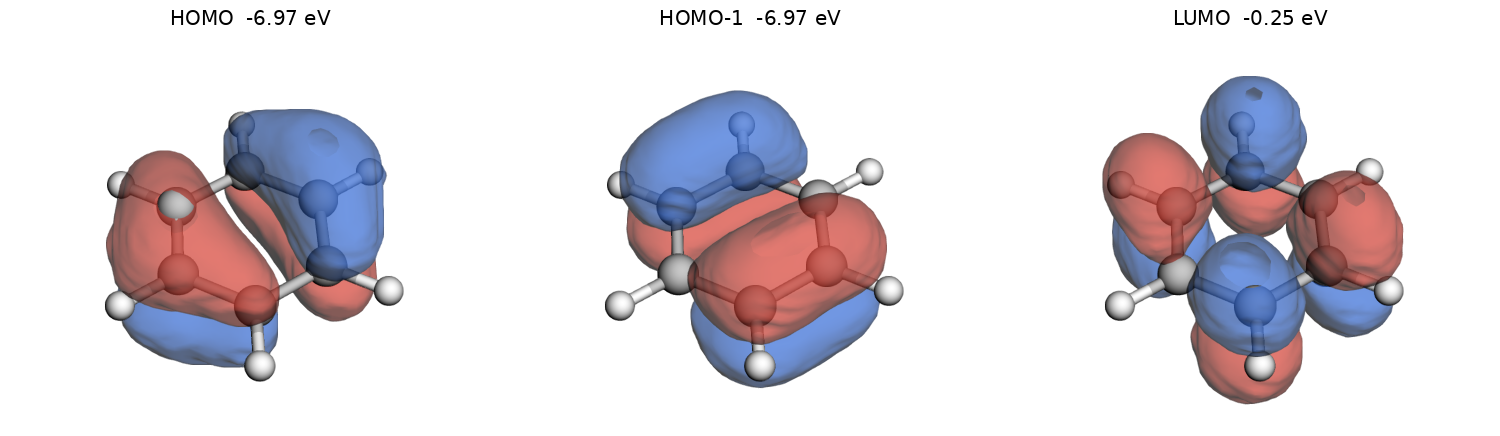
\includegraphics[width=0.72\linewidth]{benzene_frontier.png}
\caption{Frontier orbitals of benzene (B3LYP/def2-SVP; isosurfaces at $\pm$0.03~a.u.). HOMO and
HOMO$-1$ form the degenerate $e_{1g}$ pair; the LUMO belongs to the degenerate $e_{2u}$ pair.}
\label{fig:benzene}
\end{figure}

\paragraph{Ionisation energy.} Table~\ref{tab:ie} compares the two estimates of
Eq.~\eqref{eq:ie} with experiment. The B3LYP Koopmans estimate underestimates the ionisation
energy by 2.27~eV, whereas the $\Delta$SCF value agrees with experiment to within 0.01~eV. The
discrepancy is due to the self-interaction error of approximate exchange--correlation
functionals. The Hartree (Coulomb) term includes each electron's interaction with its own density,
and approximate functionals cancel this only partially. The remaining spurious self-repulsion
destabilises occupied orbitals and raises $\varepsilon_\text{HOMO}$. $\Delta$SCF avoids orbital
energies entirely. It uses differences of total energies, in which much of the error cancels, and
it includes the relaxation of the remaining electrons after ionisation. The HF Koopmans value
(9.17~eV) is also close to experiment. HF has no self-interaction error, and its two main
omissions, orbital relaxation (which makes the IE too large) and electron correlation (which makes
it too small), partly cancel.

\begin{table}[h]
\centering\small
\caption{Vertical ionisation energy of benzene (def2-SVP).}
\label{tab:ie}
\begin{tabular}{@{}lrr@{}}
\toprule
Method & IE (eV) & Deviation (eV) \\
\midrule
Experiment & 9.24 & --- \\
$-\varepsilon_\text{HOMO}$, B3LYP & 6.97 & $-2.27$ \\
$-\varepsilon_\text{HOMO}$, HF & 9.17 & $-0.07$ \\
$\Delta$SCF, B3LYP (UKS cation) & 9.24 & $0.00$ \\
\bottomrule
\end{tabular}
\end{table}

\paragraph{Excitation energies.} Table~\ref{tab:td} lists the lowest TDDFT excitations. The
$S_1$ and $S_2$ states have zero oscillator strength: they are symmetry-forbidden at the $D_{6h}$
geometry. This is consistent with the weak experimental band at 254~nm (4.9~eV), which gains
intensity only through vibronic coupling. The first allowed transition (degenerate $S_3$/$S_4$,
$f = 0.59$) lies at 7.28~eV, compared with about 6.9~eV experimentally. The TDDFT errors of
0.4--0.6~eV are somewhat larger than the $\approx$0.3~eV typical of hybrid functionals over
large benchmark sets~\cite{jacquemin2009}, as expected for a small double-$\zeta$ basis.
The Kohn--Sham HOMO--LUMO gap (6.72~eV) differs from the lowest excitation by 1.2~eV and contains
no information about which transitions are allowed.

\begin{table}[h]
\centering\small
\caption{Lowest TDDFT singlet excitations of benzene (B3LYP/def2-SVP) compared with the
Kohn--Sham gap and experiment.}
\label{tab:td}
\begin{tabular}{@{}lrrrl@{}}
\toprule
& $E$ (eV) & $\lambda$ (nm) & $f$ & Experiment \\
\midrule
KS gap, $\varepsilon_\text{LUMO}-\varepsilon_\text{HOMO}$ & 6.72 & 184 & --- & --- \\
$S_1$ & 5.48 & 226 & 0.000 & 4.9~eV (254~nm), weak \\
$S_2$ & 6.22 & 199 & 0.000 & --- \\
$S_3$, $S_4$ & 7.28 & 170 & 0.589 & $\approx$6.9~eV, strong \\
\bottomrule
\end{tabular}
\end{table}

These results separate three quantities that are often confused. The \emph{Kohn--Sham gap} is a
difference of orbital eigenvalues. The \emph{fundamental gap}, $\mathrm{IE}-\mathrm{EA}$, refers to
removing and adding an electron in separate systems. The \emph{optical gap} is the lowest neutral
excitation, which is lowered relative to the fundamental gap by the electron--hole attraction.
Only the optical gap corresponds to an absorption spectrum, and it requires an excited-state method
such as TDDFT.

\subsection{From SMILES to a DFT calculation}

An RDKit molecule constructed from a SMILES string is a molecular graph. It contains atoms, bonds,
formal charges and implicit hydrogen counts, but no Cartesian coordinates. DFT, in contrast,
requires only nuclear positions, total charge and spin multiplicity, together with the choice of
method. Explicit hydrogens, ETKDG embedding and MMFF94 relaxation bridge the two.
For benzene this route gave $r$(C--C) = 1.395~\AA, and a HOMO energy within 0.008~eV of that at the
DFT-optimised geometry.

Table~\ref{tab:aq} shows the corresponding results for anthraquinone (\ce{C14H8O2}; 108 electrons,
264 basis functions). The geometry (MMFF94 versus DFT-optimised) shifts both frontier orbitals by
0.02--0.03~eV in the same direction, so the gap changes by only 0.007~eV. Implicit water shifts the
HOMO by $-0.12$~eV and the gap by $+0.07$~eV. These effects are small because anthraquinone is
rigid, has a single low-energy conformer, and is neutral with a negligible dipole moment.

\begin{table}[h]
\centering\small
\caption{Frontier-orbital energies of anthraquinone (B3LYP/def2-SVP).}
\label{tab:aq}
\begin{tabular}{@{}llrrr@{}}
\toprule
Geometry & Solvent & $\varepsilon_\text{HOMO}$ (eV) & $\varepsilon_\text{LUMO}$ (eV) & Gap (eV) \\
\midrule
MMFF94 & vacuum & $-7.170$ & $-2.976$ & 4.194 \\
MMFF94 & water (ddCOSMO) & $-7.288$ & $-3.022$ & 4.266 \\
DFT-optimised & water (ddCOSMO) & $-7.314$ & $-3.041$ & 4.273 \\
\bottomrule
\end{tabular}
\end{table}

A practical point concerns the charge. PySCF can read Cartesian coordinates directly from an xyz
file, but the xyz format has no charge field. When the eosin~Y dianion's structure file was read
this way, the molecule was assigned charge 0 and 306 electrons instead of 308, without any warning.
The total charge must therefore always be supplied explicitly.

\subsection{Effect of charge and implicit solvation}

Phenol and its conjugate base, phenolate, were used as minimal models of the deprotonated phenol
oxygen found in eosin~Y and related xanthene dyes (Table~\ref{tab:phenol}). In vacuum the phenolate
HOMO is positive ($+0.32$~eV): the excess electron is unbound at this level of theory. The absence
of diffuse basis functions and self-interaction error both contribute to this. Implicit water
lowers the phenolate HOMO by 4.47~eV, compared with only 0.08~eV for neutral phenol, because the
dielectric continuum responds mainly to the net charge.

\begin{table}[h]
\centering\small
\caption{HOMO energies of phenol and phenolate in vacuum and in implicit water (B3LYP/def2-SVP,
MMFF94 geometries).}
\label{tab:phenol}
\begin{tabular}{@{}lrrr@{}}
\toprule
& $\varepsilon_\text{HOMO}$, vacuum (eV) & $\varepsilon_\text{HOMO}$, water (eV) & Shift (eV) \\
\midrule
Phenol, \ce{C6H5OH} & $-6.18$ & $-6.26$ & $-0.08$ \\
Phenolate, \ce{C6H5O-} & $+0.32$ & $-4.15$ & $-4.47$ \\
\bottomrule
\end{tabular}
\end{table}

When phenolate was built with the default charge of zero, the calculation was rejected because 49
electrons cannot form a closed-shell singlet. For a dianion, omitting the charge removes two
electrons, leaving an even electron count. The calculation then runs without error on the wrong
species, as in the eosin~Y example above.

\subsection{Reproduction of a photocatalyst-workflow result}

A single-point calculation written independently, using the procedure of the preceding sections,
was run on the workflow's B3LYP/def2-SVP-optimised anthraquinone geometry in implicit water. It gave
$\varepsilon_\text{HOMO} = -7.3138$~eV and $\varepsilon_\text{LUMO} = -3.0409$~eV, identical to the
workflow's stored values to four decimal places. This confirms that the workflow's frontier-orbital
step performs the calculation described here.

%=============================================================================
\section{Implications for the Photocatalyst Study}

\begin{enumerate}
  \item \textbf{Frontier-orbital energies.} The B3LYP HOMO and LUMO energies of the 16
  photocatalysts are shifted by self-interaction error of the order of 2~eV (Table~\ref{tab:ie}).
  They can be used to compare molecules and identify trends, but not as absolute ionisation
  energies, electron affinities or redox potentials. Plotting them against the water-splitting
  redox levels is therefore not justified. Redox potentials should instead be computed as
  $\Delta$SCF free-energy differences in solvent.
  \item \textbf{Optical properties.} The study's current comparison of the Kohn--Sham gap with the
  lowest experimental absorption band measures a trend, not absorption energies. Excitation
  energies, oscillator strengths and the character of each excitation require TDDFT. A
  range-separated functional is advisable for the charge-transfer catalysts (Mes-Acr$^+$, 4CzIPN).
  \item \textbf{Geometry.} For rigid, neutral molecules, MMFF94 geometries change the frontier
  orbitals by only about 0.01~eV. Flexible or charged dyes require separate verification.
  \item \textbf{Charge and solvation.} The dianionic and cationic dyes must carry their charge
  explicitly and be treated with a solvent model. Using the same implicit solvent for all 16
  molecules keeps the level of theory consistent, so they can be compared directly. For neutral,
  non-polar molecules this has little effect; for strongly polar neutral molecules, such as
  riboflavin, it may matter more.
\end{enumerate}

%=============================================================================
\section{Conclusions}

Benchmark calculations on small reference molecules have established the behaviour of the
B3LYP/def2-SVP/ddCOSMO level of theory used in the photocatalyst study. Geometries are accurate to
about 0.01~\AA. $\Delta$SCF reproduces the ionisation energy of benzene, while the Kohn--Sham HOMO
underestimates it by 2.27~eV. TDDFT correctly identifies the lowest singlet excitation of benzene
as dark, and it lies 1.2~eV below the Kohn--Sham gap. Implicit solvation is essential for anions
(4.47~eV stabilisation of the phenolate HOMO) but has little effect on neutral, non-polar molecules.
An independent calculation reproduced the workflow's frontier-orbital energies for anthraquinone
exactly. The next steps are to add TDDFT excitation energies to the photocatalyst study, beginning
with anthraquinone (experimental absorption at 325~nm), and to verify the frontier orbitals of the
flexible dyes at their DFT-optimised geometries.

%=============================================================================
\begin{thebibliography}{99}\small
\bibitem{romero2016} N.~A. Romero and D.~A. Nicewicz, \emph{Chem.\ Rev.} \textbf{116}, 10075 (2016).
\bibitem{pyscf2020} Q. Sun \emph{et al.}, \emph{J.\ Chem.\ Phys.} \textbf{153}, 024109 (2020).
\bibitem{becke1993} A.~D. Becke, \emph{J.\ Chem.\ Phys.} \textbf{98}, 5648 (1993).
\bibitem{lee1988} C. Lee, W. Yang and R.~G. Parr, \emph{Phys.\ Rev.\ B} \textbf{37}, 785 (1988).
\bibitem{weigend2005} F. Weigend and R. Ahlrichs, \emph{Phys.\ Chem.\ Chem.\ Phys.} \textbf{7}, 3297 (2005).
\bibitem{cances2013} E. Canc\`es, Y. Maday and B. Stamm, \emph{J.\ Chem.\ Phys.} \textbf{139}, 054111 (2013).
\bibitem{wang2016} L.-P. Wang and C. Song, \emph{J.\ Chem.\ Phys.} \textbf{144}, 214108 (2016).
\bibitem{riniker2015} S. Riniker and G.~A. Landrum, \emph{J.\ Chem.\ Inf.\ Model.} \textbf{55}, 2562 (2015).
\bibitem{halgren1996} T.~A. Halgren, \emph{J.\ Comput.\ Chem.} \textbf{17}, 490 (1996).
\bibitem{koopmans1934} T. Koopmans, \emph{Physica} \textbf{1}, 104 (1934).
\bibitem{jacquemin2009} D. Jacquemin, V. Wathelet, E.~A. Perp\`ete and C. Adamo, \emph{J.\ Chem.\
  Theory Comput.} \textbf{5}, 2420 (2009).
\end{thebibliography}

\end{document}
